\documentclass[10pt,a4paper]{article}
\usepackage[utf8]{inputenc}
\usepackage[T1]{fontenc}
\usepackage[spanish,es-tabla]{babel}
\usepackage[margin=2cm]{geometry}
\usepackage{booktabs}
\usepackage{graphicx}
\usepackage{listings}
\lstset{basicstyle=\ttfamily\footnotesize,breaklines=true,columns=fullflexible}
\setlength{\parindent}{0pt}
\setlength{\parskip}{0.4em}

\begin{document}

\section{Construcción de supercalibraciones (Paso 4)}

\subsection{Las tareas de combinación de IRAF y su dependencia de las cabeceras}

Las tareas del paquete \texttt{ccdred} utilizadas para construir supercalibraciones son:

\begin{itemize}
\item \textbf{imcombine}: motor general de combinación. Promedia (o mediana/suma) píxel a píxel un conjunto de imágenes con algoritmos de rechazo de atípicos (\texttt{avsigclip}, \texttt{minmax}, \texttt{pclip}); no interpreta cabeceras CCD por sí misma.
\item \textbf{zerocombine}: envoltorio de \texttt{imcombine} especializado en marcos de nivel cero; combina los bias sin escalado temporal (\texttt{scale=none}), pues su exposición es despreciable.
\item \textbf{darkcombine}: combina imágenes oscuras y puede escalarlas por tiempo de exposición (\texttt{scale=exposure}) para llevarlas al tiempo de la ciencia antes de promediar.
\item \textbf{flatcombine}: combina campos planos; normaliza cada marco (por moda o mediana) y puede agrupar por filtro (\texttt{subset}), de modo que el master flat resultante tenga nivel medio unidad.
\end{itemize}

\noindent\textbf{¿Requieren parámetros de las cabeceras?} Sí. Los envoltorios
leen \texttt{IMAGETYP} (parámetro \texttt{ccdtype}) para seleccionar los marcos
del tipo pedido, \texttt{EXPTIME} para el escalado temporal de darks y
\texttt{FILTER} para agrupar flats por banda. En este trabajo las listas de
entrada se construyeron explícitamente por tipo
(\texttt{lista\_bias.txt}, \texttt{lista\_dark.txt},
\texttt{lista\_flat\_B.txt}, \texttt{lista\_flat\_V.txt}), por lo que el
filtrado por cabecera no fue necesario; además, en esta compilación
(Community IRAF 2.17.1) las tareas \texttt{darkcombine} y \texttt{flatcombine}
reportaron errores de archivo de parámetros, así que la combinación
equivalente se realizó con \texttt{imcombine}, fijando manualmente el escalado
(\texttt{scale=none} para darks, \texttt{scale=mode} para flats). Otra nota
técnica: en ECL la sintaxis de listas \texttt{@archivo} solo es válida como
valor de un parámetro (\texttt{input=@lista}), no como argumento posicional.

\subsection{Master bias (Paso 4a)}

Se combinaron los 48 marcos de nivel cero ya corregidos de overscan
(47 bias + \texttt{LbTrmZero.fits}) con rechazo sigma iterativo:

\begin{lstlisting}
noao
imred
ccdred
unlearn zerocombine
!ls LbTrmdomeflat_Bias_1_secs_*.fits LbTrmZero.fits > lista_bias.txt
zerocombine input=@lista_bias.txt output=MasterBias.fits \
  combine=average reject=avsigclip scale=none
imhead MasterBias.fits
imstat MasterBias.fits
display MasterBias.fits 1 fill+ zscale-
\end{lstlisting}

\noindent El master bias resulta con media $\approx 0.26$ ADU, es decir, nivel
de lectura efectivamente removido por la corrección de overscan. Su
desviación de 2.36 ADU se descompone en el componente aleatorio
$\sigma_{\mathrm{marco}}/\sqrt{48} = 6.64/6.93 \approx 0.96$ ADU más un
patrón fijo de columnas ($\approx 2.15$ ADU) idéntico en todos los marcos, que
el promedio no elimina y que se aprecia como rayas verticales en DS9
(rango z: $-7.8$ a $15.5$ ADU). El máximo de 1509 ADU corresponde a píxeles
calientes presentes en los 48 marcos: al no ser atípicos dentro del stack,
\texttt{avsigclip} los conserva.

\subsection{Master dark (Paso 4b)}

Se combinaron los 5 darks de 90 s corregidos de overscan. Como todos comparten
idéntico tiempo de exposición, el escalado por \texttt{EXPTIME} es innecesario
(\texttt{scale=none}):

\begin{lstlisting}
!ls LbTrmMEL25_Dark_90_secs_*.fits > lista_dark.txt
imcombine input=@lista_dark.txt output=MasterDark.fits \
  combine=average reject=avsigclip scale=none
imhead MasterDark.fits
imstat MasterDark.fits
display MasterDark.fits 2 fill+ zscale-
\end{lstlisting}

\noindent La media del master dark es 0.36 ADU en 90 s
($\approx 0.004$ ADU/s $\approx 0.006$ e$^-$/s con $g=1.45$): a
$-25\,^{\circ}$C la corriente oscura del CCD-FLI ML0900 es despreciable, de
modo que la corrección de dark es marginal pero se aplica por rigor
metodológico. La desviación de 49.6 ADU y el máximo de 64526 ADU están
dominados por píxeles calientes persistentes (visible en DS9 como puntos
blancos aislados sobre fondo negro, rango z: $-15.7$ a $571.5$); el
componente aleatorio esperado es $6.64/\sqrt{5} \approx 2.97$ ADU.

\subsection{Master flats por filtro (Paso 4c)}

Cada dome flat se inspeccionó individualmente en DS9
(\texttt{display ... fill+ zscale-}): los cinco marcos por filtro muestran un
gradiente de iluminación suave y reproducible, sin estrellas superpuestas ni
píxeles saturados (máximos $\sim 1.6\times10^{4}$ ADU, muy por debajo del
techo de 65535 del formato ushort), por lo que ningún marco fue descartado.
Se combinaron con \texttt{scale=mode}, que iguala las modas de los marcos
antes de promediar (factores de escala entre 0.995 y 1.006, Tabla~\ref{tab:modes}):

\begin{lstlisting}
!ls LbTrmdomeflat_Flat_B_90_secs_*.fits > lista_flat_B.txt
imcombine input=@lista_flat_B.txt output=MasterFlat_B.fits \
  combine=average reject=avsigclip scale=mode
!ls LbTrmdomeflat_Flat_V_40_secs_*.fits > lista_flat_V.txt
imcombine input=@lista_flat_V.txt output=MasterFlat_V.fits \
  combine=average reject=avsigclip scale=mode
\end{lstlisting}

\begin{table}[ht]
\centering
\caption{Modas y factores de escala aplicados por \texttt{imcombine}
(\texttt{scale=mode}) a cada dome flat.}
\label{tab:modes}
\footnotesize
\begin{tabular}{lcc|lcc}
\toprule
Marco (B) & Moda (ADU) & Escala & Marco (V) & Moda (ADU) & Escala \\
\midrule
Flat\_B\_001 & 13716 & 1.000 & Flat\_V\_001 & 13547 & 1.000 \\
Flat\_B\_002 & 13741 & 0.998 & Flat\_V\_002 & 13568 & 0.998 \\
Flat\_B\_003 & 13786 & 0.995 & Flat\_V\_003 & 13593 & 0.997 \\
Flat\_B\_004 & 13775 & 0.996 & Flat\_V\_004 & 13585 & 0.997 \\
Flat\_B\_005 & 13767 & 0.996 & Flat\_V\_005 & 13471 & 1.006 \\
\bottomrule
\end{tabular}
\end{table}

\noindent Siguiendo las notas, cada master flat se normalizó dividiéndolo por
su valor representativo (moda); se verificó que las modas individuales
(13471--13786 ADU) coinciden con la media del master dentro de aproximadamente un 2 por ciento,
por lo que se adoptó como divisor la media reportada por \texttt{imstat}
(13458 en B y 13177 en V), lo que fija la media del flat normalizado en
1.000 sin alterar su forma espacial:

\begin{lstlisting}
imarith MasterFlat_B.fits / 13458. MasterFlat_B_norm.fits
imarith MasterFlat_V.fits / 13177. MasterFlat_V_norm.fits
imstat MasterFlat_B_norm.fits
imstat MasterFlat_V_norm.fits
\end{lstlisting}

\noindent Los flats normalizados presentan media exactamente 1.000 y
desviación de 0.076 (B) y 0.079 (V): esa dispersión relativa entre
7.6 y 7.9 por ciento corresponde al gradiente de iluminación del domo y el viñeteo
que la división transferirá como corrección de sensibilidad píxel a píxel.
Los mínimos (0.013 y 0.007) marcan esquinas fuertemente viñeteadas o motas de
polvo; los máximos (4.77 y 4.88) son defectos residuales presentes en todos
los marcos del conjunto.

\subsection{Resumen estadístico e inspección visual (Entregable 4)}

La Tabla~\ref{tab:masters} resume las estadísticas de \texttt{imstat} de las
cuatro supercalibraciones y de los flats normalizados; la
Figura~\ref{fig:masters} muestra la inspección visual simultánea en DS9.

\begin{table}[ht]
\centering
\caption{Estadísticas de \texttt{imstat} de las supercalibraciones
(9\,171\,756 píxeles cada una, [3021,3036]).}
\label{tab:masters}
\footnotesize
\begin{tabular}{lrrrrr}
\toprule
Imagen & $N_{\mathrm{marcos}}$ & Media (ADU) & Desv. (ADU) & Mín & Máx \\
\midrule
MasterBias          & 48 & 0.2641 & 2.358   & $-23.83$ & 1509    \\
MasterDark          & 5  & 0.3645 & 49.57   & $-33.37$ & 64526   \\
MasterFlat\_B       & 5  & 13458  & 1019    & 171.5    & 64137   \\
MasterFlat\_V       & 5  & 13177  & 1040    & 95.41    & 64293   \\
MasterFlat\_B\_norm & 5  & 1.000  & 0.0757  & 0.01274  & 4.766   \\
MasterFlat\_V\_norm & 5  & 1.000  & 0.07894 & 0.007241 & 4.879   \\
\bottomrule
\end{tabular}
\end{table}

\begin{figure}[ht]
\centering
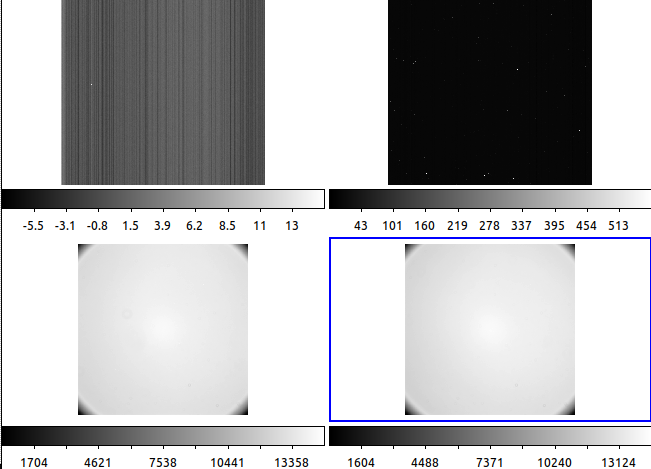
\includegraphics[width=0.95\linewidth]{imagenes/supercalibraciones_ds9.png}
\caption{Inspección visual en DS9 (\texttt{fill+ zscale-}) de las cuatro
supercalibraciones. Arriba: MasterBias (patrón fijo de columnas,
z: $-7.8$ a $15.5$ ADU) y MasterDark (fondo negro con píxeles calientes,
z: $-15.7$ a $571.5$ ADU). Abajo: MasterFlat\_B (z: $252.2$ a $14810$) y
MasterFlat\_V (z: $169.4$ a $14559$), con el gradiente de iluminación del
domo y viñeteo en esquinas.}
\label{fig:masters}
\end{figure}

\noindent\textbf{Lectura conjunta.} El master bias confirma que la corrección
de overscan dejó el nivel de lectura en cero y que el ruido aleatorio se
redujo por $\sqrt{48}$; el master dark demuestra que a $-25\,^{\circ}$C la
corriente oscura es despreciable frente al ruido de lectura; y los master
flats normalizados conservan únicamente la respuesta relativa del sistema
(iluminación del domo, viñeteo y polvo), lista para dividir las imágenes de
ciencia sin alterar su flujo absoluto.

\end{document}